\chapter{Problem 2: Dua Nakhoda, Satu Kapal (Orang 1, load test: Orang 2)}

> Draf bagian laporan M2 (Markdown, laporan final dikompilasi ke PDF). Bukti: \texttt{make demo-\allowbreak{}m2-\allowbreak{}p2} > (\texttt{docs/\allowbreak{}evidence/\allowbreak{}m2/\allowbreak{}p2-\allowbreak{}latest.\allowbreak{}log}), \texttt{bash scripts/\allowbreak{}demo/\allowbreak{}m2-\allowbreak{}single-\allowbreak{}writer.\allowbreak{}sh}, \texttt{bash scripts/\allowbreak{}demo/\allowbreak{}m2-\allowbreak{}freeze.\allowbreak{}sh}, > \texttt{bash scripts/\allowbreak{}k8s/\allowbreak{}practice.\allowbreak{}sh clock-\allowbreak{}skew|\allowbreak{}kill-\allowbreak{}leader}, dan test \texttt{services/\allowbreak{}aggregator/\allowbreak{}internal/\allowbreak{}leader}, > \texttt{internal/\allowbreak{}ports/\allowbreak{}repotest} (\texttt{run\allowbreak{}Fence}).


\section{Identifikasi masalah}

{\small
\begin{longtable}{@{}>{\raggedright\arraybackslash}p{0.112\linewidth}>{\raggedright\arraybackslash}p{0.411\linewidth}>{\raggedright\arraybackslash}p{0.411\linewidth}@{}}
\toprule
\textbf{Kriteria} & \textbf{Persoalan} & \textbf{Nama dalam literatur} \\
\midrule
\endhead
2 & Tiga instance identik sama-sama menjalankan polling, sehingga setiap kejadian diambil dan dicatat tiga kali & \emph{Leader election} / \emph{mutual exclusion} terdistribusi, konsumsi \emph{exactly-once} dari sumber pull \\
4 & Pemegang tugas ditentukan dengan ``masa berlaku'' berbasis waktu, padahal jam tiap mesin bisa melompat (NTP mati, +45 s / --30 s) & \emph{Clock skew} dan \emph{clock drift}, tidak ada \emph{global clock}, asumsi \emph{bounded clock error} pada \emph{lease} (Gray \& Cheriton 1989) \\
5 & Proses yang dibekukan (VM di-\emph{suspend}, laptop ditutup) bangun dan melanjutkan pekerjaannya karena merasa masih pemimpin & \emph{Process pause} (GC/VM pause) dan \emph{zombie leader}, diatasi dengan \emph{fencing token} (Kleppmann, \emph{How to do distributed locking}, 2016, DDIA bab 8) \\
\bottomrule
\end{longtable}
}

Inti persoalan: di sistem terdistribusi tidak ada cara bagi sebuah proses untuk \textbf{tahu} bahwa ia masih pemimpin pada saat ia menulis. Sebuah \emph{lease} hanya memberi tahu bahwa ia pemimpin \textbf{ketika lease terakhir dibaca}. Jeda apa pun di antara membaca dan menulis (GC, \emph{suspend}, jaringan) membuka celah dua pemimpin.


\section{Rancangan solusi}

\begin{figure}[H]\centering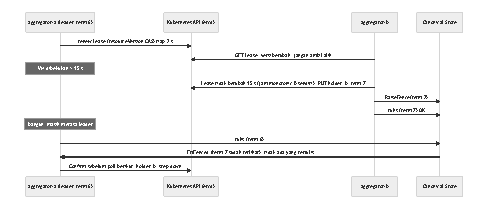
\includegraphics[width=\linewidth,height=0.82\textheight,keepaspectratio]{fig/m4.pdf}\end{figure}

\begin{enumerate}
\item \textbf{Satu penulis lewat leader election} (\texttt{services/\allowbreak{}aggregator/\allowbreak{}internal/\allowbreak{}leader}). Semua instance melayani baca, hanya pemegang Lease \texttt{aggregator-\allowbreak{}ingest} yang menjalankan polling BMKG/PVMBG, relay outbox, dan retry dead letter. Implementasinya klien REST kecil ke API Kubernetes (tanpa client-go): \texttt{GET}, lalu \texttt{POST}/\texttt{PUT} dengan \texttt{resource\allowbreak{}Version} sebagai \emph{compare-and-swap}, sehingga etcd yang mengurutkan semua perubahan.
\item \textbf{Term = token fencing.} Setiap pergantian pemegang menaikkan \texttt{lease\allowbreak{}Transitions}. Konteks kerja leader membawa \texttt{ports.\allowbreak{}Fence\{Name,\allowbreak{} Term,\allowbreak{} Holder\}} dan setiap tulis ke store (\texttt{Save}, \texttt{Set\allowbreak{}Cursor}, dead letter, status sumber) memeriksanya \textbf{di dalam transaksi yang sama} dengan tulisnya (\texttt{adapters/\allowbreak{}postgres/\allowbreak{}unprocessed.\allowbreak{}go}, \texttt{check\allowbreak{}Fence}): baris \texttt{fence} dikunci, term yang lebih kecil dari yang tersimpan ditolak (\texttt{Err\allowbreak{}Fenced}, transaksi di-\emph{rollback}), term yang lebih besar menaikkan nilai tersimpan. Leader baru memanggil \texttt{Raise\allowbreak{}Fence} sebelum tulis pertamanya, karena kunci baris, tulis term lama yang sedang berjalan selesai lebih dulu, dan setiap tulis term lama sesudahnya ditolak.
\item \textbf{Gerbang sebelum memanggil upstream} (\texttt{Loop.\allowbreak{}Gate} = \texttt{Elector.\allowbreak{}Confirm}): sebelum setiap siklus poll, leader membaca ulang Lease. Leader yang baru bangun dari \emph{freeze} langsung tahu ia sudah diganti dan mundur, jadi BMKG/PVMBG tidak menerima permintaan dari dua instance. Header \texttt{X-\allowbreak{}Caller} (nama pod) membuat hal ini terlihat di log upstream.
\item \textbf{Status sumber dibagi lewat store} (\texttt{Put\allowbreak{}Source\allowbreak{}Status}): instance yang tidak polling tetap memberi \texttt{freshness} yang benar. Umur status diukur dengan jam store, status yang tidak diperbarui > 30 s ditandai \texttt{unknown} + \texttt{stale\_\allowbreak{}since}.
\item \textbf{Titik masuk dan rolling update} (\texttt{deploy/\allowbreak{}k8s/\allowbreak{}aggregator.\allowbreak{}yaml}): Service Kubernetes di depan $\ge$ 3 replika dengan \texttt{topology\allowbreak{}Spread\allowbreak{}Constraints} (maxSkew 1 per node), \texttt{readiness\allowbreak{}Probe /\allowbreak{}ready} tiap 2 s (instance yang tidak bisa menjangkau store keluar dari Service setelah 4 s), \texttt{max\allowbreak{}Unavailable: 0}, \texttt{pre\allowbreak{}Stop sleep 10}, dan \emph{graceful shutdown}: permintaan yang sedang berjalan diselesaikan (konteks request tidak ikut dibatalkan SIGTERM), leader melepas Lease saat berhenti sehingga penggantinya mengambil alih dalam $\pm$2 s, bukan 15 s.
\end{enumerate}

\section{Sumber kebenaran waktu (jawaban hint)}

\textbf{Tidak ada jam yang dipercaya untuk keselamatan (safety).} Keputusan ``siapa boleh menulis'' diambil oleh store dari urutan term, bukan dari waktu. Waktu hanya dipakai untuk \textbf{liveness} (kapan mengambil alih), dan itu pun tanpa membandingkan jam dua mesin:


\begin{itemize}
\item Urutan perubahan Lease ditentukan oleh etcd (\texttt{resource\allowbreak{}Version}), satu tempat.
\item Kandidat menganggap Lease kedaluwarsa bila objek Lease \textbf{tidak berubah} selama \texttt{LEASE\_\allowbreak{}DURATION\_\allowbreak{}SEC} menurut \textbf{jam monotonic kandidat sendiri}, dihitung sejak ia pertama kali melihat versi itu. \texttt{renew\allowbreak{}Time} di objek (ditulis dengan jam dinding pemegang) tidak pernah dibaca untuk keputusan. Jam dinding yang melompat +45 s / --30 s tidak menggeser jam monotonic.
\item Leader berhenti sendiri bila gagal memperbarui selama \texttt{RENEW\_\allowbreak{}DEADLINE} (10 s) < \texttt{LEASE\_\allowbreak{}DURATION} (15 s), lagi-lagi dengan jam monotonic-nya. Selisih 5 s itu memastikan, selama laju jam kedua mesin wajar, leader lama sudah berhenti sebelum penerus boleh mengambil alih.
\item Bila asumsi itu dilanggar (VM dibekukan: jam monotonic tidak berjalan), \textbf{fencing} di store tetap mencegah tulis ganda. Waktu tulis untuk audit (\texttt{outbox.\allowbreak{}stored\_\allowbreak{}at}) diambil dari jam store, satu jam untuk semua penulis.
\end{itemize}

Kenapa aman pada kriteria 4: pergeseran jam tidak mengubah keputusan siapa pun (lihat \texttt{Test\allowbreak{}Skewed\allowbreak{}Holder\allowbreak{}Clock\allowbreak{}Does\allowbreak{}Not\allowbreak{}Cause\allowbreak{}Takeover}, \texttt{Test\allowbreak{}Clock\allowbreak{}Jump\allowbreak{}On\allowbreak{}Leader\allowbreak{}Node\allowbreak{}Keeps\allowbreak{}Single\allowbreak{}Leader}). Kenapa aman pada kriteria 5: leader yang bangun memegang term lama, penerusnya sudah menaikkan fence, jadi semua tulisnya ditolak store, dan \texttt{Confirm} membuatnya mundur sebelum poll berikutnya (\texttt{Test\allowbreak{}Frozen\allowbreak{}Leader\allowbreak{}Is\allowbreak{}Fenced\allowbreak{}After\allowbreak{}Waking\allowbreak{}Up}, di cluster: \texttt{scripts/\allowbreak{}demo/\allowbreak{}m2-\allowbreak{}freeze.\allowbreak{}sh} memeriksa \texttt{SELECT count(*) FROM outbox WHERE writer\_\allowbreak{}term =\allowbreak{} <term lama> AND stored\_\allowbreak{}at > <awal freeze>} = 0).


\section{Batas waktu dan trade-off}

{\small
\begin{longtable}{@{}>{\raggedright\arraybackslash}p{0.173\linewidth}>{\raggedright\arraybackslash}p{0.179\linewidth}>{\raggedright\arraybackslash}p{0.582\linewidth}@{}}
\toprule
\textbf{Parameter} & \textbf{Nilai} & \textbf{Alasan dan trade-off} \\
\midrule
\endhead
\texttt{LEASE\_\allowbreak{}DURATION\_\allowbreak{}SEC} & 15 s & Waktu ambil alih terburuk $\approx$ 15 s + 2 s (retry) + 3 s (siklus poll) $\approx$ 20 s, jauh di bawah 60 s. Lebih kecil = failover lebih cepat tetapi jeda GC / jaringan sesaat bisa memicu pergantian leader yang tidak perlu. \\
\texttt{LEASE\_\allowbreak{}RENEW\_\allowbreak{}DEADLINE\_\allowbreak{}SEC} & 10 s & Leader menyerah 5 s sebelum orang lain boleh mengambil alih: margin untuk perbedaan laju jam. \\
\texttt{LEASE\_\allowbreak{}RETRY\_\allowbreak{}PERIOD\_\allowbreak{}SEC} & 2 s & 5 kali kesempatan renew dalam satu deadline, beban API server $\approx$ 1 permintaan / 2 s per instance. \\
\texttt{Confirm} sebelum tiap poll & 1 GET Lease / siklus / sumber & Biaya kecil, menutup celah ``bangun lalu langsung memanggil upstream''. \\
Toleransi node \texttt{unreachable} & 20 s & Pod di node mati diganti setelah 20 s (bawaan 300 s). Terlalu kecil = pod dipindah karena gangguan jaringan singkat. \\
\texttt{SOURCE\_\allowbreak{}STATUS\_\allowbreak{}MAX\_\allowbreak{}AGE\_\allowbreak{}SEC} & 30 s & > durasi lease + beberapa siklus, status yang lebih tua berarti tidak ada yang polling. \\
readiness & tiap 2 s, gagal 2$\times$ & Instance tidak sehat keluar dari Service dalam $\pm$4 s. \\
\bottomrule
\end{longtable}
}

\section{Alternatif yang dipertimbangkan}

{\small
\begin{longtable}{@{}>{\raggedright\arraybackslash}p{0.429\linewidth}>{\raggedright\arraybackslash}p{0.517\linewidth}@{}}
\toprule
\textbf{Alternatif} & \textbf{Ditolak karena} \\
\midrule
\endhead
Lock di PostgreSQL (\texttt{pg\_\allowbreak{}try\_\allowbreak{}advisory\_\allowbreak{}lock} / tabel lease dengan \texttt{now()} DB) & Mengikat koordinasi ke store yang di M2 di-\emph{shard} dan node-nya boleh mati (P1), Lease di etcd hidup di control plane yang tidak dimatikan skenario. \\
client-go \texttt{leaderelection} & Benar secara konsep, tetapi menambah dependensi besar, perilakunya sama (CAS + jam monotonic). Kami tetap butuh fencing karena client-go sendiri menyatakan tidak menjamin satu leader saat proses dijeda. \\
Partisi kerja per sumber tanpa leader (hash sumber ke instance) & Tetap perlu kesepakatan keanggotaan, rebalancing saat skala 3 $\rightarrow$ 5 $\rightarrow$ 2 menimbulkan periode dua pemilik. \\
Idempotensi saja (biarkan tiga instance polling, dedup di store) & Store memang idempoten (hazard\_id deterministik), tetapi upstream menerima permintaan berlipat (dilarang kriteria 2) dan versi hazard bisa saling timpa. \\
\bottomrule
\end{longtable}
}

\section{Batasan yang disadari}

\begin{itemize}
\item Fencing hanya melindungi unit penyimpanan yang \textbf{sudah melihat} term baru. \texttt{Raise\allowbreak{}Fence} menaikkan fence di ketiga shard sebelum tulis pertama, dan setiap tulisan memeriksa fence di transaksinya sendiri (\texttt{repotest} \texttt{run\allowbreak{}Fence} dijalankan untuk adapter \texttt{sharded}).
\item Permintaan HTTP yang \textbf{sudah terkirim} ke upstream tepat sebelum proses dibekukan bisa selesai setelah penerus mulai, hasilnya tetap ditolak store. Log upstream mencatat waktu selesai, jadi yang dibuktikan adalah tidak ada dua caller yang aktif bersamaan setelah serah terima (lihat skrip \texttt{m2-\allowbreak{}single-\allowbreak{}writer.\allowbreak{}sh}).
\item \textbf{Kapasitas cluster demo untuk load test.} Kedua VM dan generator beban (k6) berbagi satu laptop (i5-12500H, 24 GB). Pada 3.000--10.000 VU, node-a, yang sekaligus control plane, jenuh CPU dan API server tidak menjawab. Load test kriteria 6--7 karena itu belum terbukti di perangkat keras ini. Agar sahih, pengujian ini membutuhkan generator beban di mesin lain dan control plane yang tidak ikut melayani beban aplikasi (taint \texttt{No\allowbreak{}Schedule} di node-a, atau node ketiga). Mekanisme yang diuji (scale Deployment, readiness, admisi per peran) sudah dibuktikan terpisah: rolling update di bawah beban (kriteria 8) dan prioritas Lapangan di P5.
\item Lease bergantung pada control plane. Pada topologi 2 node, kehilangan control plane menghentikan pergantian leader (bukan layanan baca). Skenario wajib hanya mematikan worker.
\item Relay outbox hanya di leader, selama serah terima ($\le$ 20 s) event menunggu di outbox, tidak hilang.
\item Polling BMKG/PVMBG memakai \emph{cursor} waktu dengan overlap 5 s (pola M1). Bila sebuah upstream di-restart lalu membuat data baru yang \textbf{bertanggal lebih tua} dari cursor tersimpan, data itu tidak terambil. Contohnya mock BMKG yang membuat 24 event seed mundur hingga 36 jam. Ini bukan celah akibat pergantian leader, karena cursor tersimpan di store dan diteruskan oleh leader berikutnya. Pemeriksaan ``tanpa celah'' di \texttt{m2-\allowbreak{}p2.\allowbreak{}sh} karena itu menilai jendela failover (event sejak 15 menit sebelum leader dimatikan). Perbaikan yang lebih kuat: deteksi restart upstream (prefix ID baru) lalu reset cursor.
\item \textbf{Commit yang sedang berjalan saat freeze.} Pada run pertama di storage sharded, dua baris term 60 tersimpan pada 13:44:49 dan 13:44:54, sesudah pod leader dibekukan (log terakhirnya 13:44:45). Keduanya adalah commit yang sudah terkirim sebelum freeze dan menunggu standby sinkron di node-b yang ikut beku. Commit itu selesai setelah Patroni mencabut status sinkron standby tersebut, dan masih \textbf{sebelum} term 61 menulis pertama kali (13:46:15). Ini tidak melanggar jaminan ``satu penulis per periode''. Pemeriksaan di \texttt{m2-\allowbreak{}freeze.\allowbreak{}sh} karena itu memakai properti yang sebenarnya: tidak ada baris term lama yang tersimpan setelah term baru menulis, pada jam shard yang sama.
\item Selama node dibekukan, API k3s di laptop ini kadang lambat, sehingga pengambilalihan bisa lebih lama dari 15 s. Ini keterbatasan virtualisasi bersarang, bukan logika lease.
\end{itemize}

\section{Bukti per kriteria}

{\small
\begin{longtable}{@{}>{\raggedright\arraybackslash}p{0.161\linewidth}>{\raggedright\arraybackslash}p{0.785\linewidth}@{}}
\toprule
\textbf{Kriteria} & \textbf{Bukti} \\
\midrule
\endhead
1 & \texttt{make demo-\allowbreak{}m2-\allowbreak{}p2} langkah 1 (\texttt{docs/\allowbreak{}evidence/\allowbreak{}m2/\allowbreak{}p2-\allowbreak{}latest.\allowbreak{}log}, k3s 2 VM, storage sharded, 22 Nov): 3 instance di 2 node (\texttt{topology\allowbreak{}Spread\allowbreak{}Constraints max\allowbreak{}Skew=\allowbreak{}1}), Service hanya mengarah ke endpoint Ready. lulus \\
2 & langkah 2--4: tepat satu leader, log BMKG/PVMBG per \texttt{caller} (header \texttt{X-\allowbreak{}Caller}) hanya berurutan per masa kepemimpinan dan tidak pernah tumpang tindih, tidak ada \texttt{(source,\allowbreak{} source\_\allowbreak{}ref\_\allowbreak{}id)} ganda di ketiga shard. lulus \\
3 & langkah 5--6: pod leader dihapus paksa (tanpa melepas lease), penerus melanjutkan ingest \textbf{31 s} setelah kill (lease 15 s, + jadwal poll), 98 event BMKG di jendela failover semuanya tersimpan (missing 0), tanpa duplikat. lulus (bukti 14 Nov dengan store tunggal: 13 s) \\
4 & \texttt{practice clock-\allowbreak{}skew} + \texttt{m2-\allowbreak{}single-\allowbreak{}writer.\allowbreak{}sh}: periode tulis per term (jam store) tidak tumpang tindih \\
5 & \texttt{m2-\allowbreak{}freeze.\allowbreak{}sh} (VM node-b di-\emph{pause} VirtualBox 40 s, storage sharded, 22 Nov, \texttt{docs/\allowbreak{}evidence/\allowbreak{}m2/\allowbreak{}freeze.\allowbreak{}log}): leader term 62 di node-b dibekukan, penerus mengambil lease dengan term 63. Setelah bangun: \textbf{0} baris term 62 tersimpan setelah term 63 menulis (diukur dengan jam masing-masing shard), \textbf{0} log \texttt{hazard\_\allowbreak{}stored} dari pod yang bangun setelah momen freeze, \texttt{m2-\allowbreak{}single-\allowbreak{}writer.\allowbreak{}sh}: tidak ada dua instance yang polling atau menyimpan pada periode yang sama. lulus \\
6 & \texttt{scripts/\allowbreak{}loadtest/\allowbreak{}m2-\allowbreak{}scale.\allowbreak{}sh} dijalankan di cluster demo (k6 v1.4.2 di laptop host, lewat NIC host-only ke NodePort kedua node). \textbf{Tidak tercapai di perangkat keras ini.} Tiga percobaan: 10.000 VU dengan jeda 1 s, 10.000 VU dengan jeda 8 s, dan 3.000 VU dengan jeda 3 s. Semuanya membuat node-a (control plane + worker, 4 vCPU) jenuh. API server berhenti menjawab (\texttt{TLS handshake timeout}), sehingga \texttt{kubectl scale} 3 $\rightarrow$ 5 gagal dan sebagian besar permintaan \emph{timeout} (12.678 permintaan gagal pada percobaan 3.000 VU). Transkrip: \texttt{docs/\allowbreak{}evidence/\allowbreak{}m2/\allowbreak{}p2-\allowbreak{}loadtest-\allowbreak{}scale-\allowbreak{}10k-\allowbreak{}attempt.\allowbreak{}log}. Lihat §6. \\
7 & \texttt{scripts/\allowbreak{}loadtest/\allowbreak{}m2-\allowbreak{}throughput.\allowbreak{}sh} siap (mode \emph{max}, CPU limit sama per pod, 1 lalu 3 instance). Pengukuran di cluster demo \textbf{tidak dilakukan} karena cluster yang sama sudah jenuh pada kriteria 6. Hasilnya tidak akan mengukur Aggregator, melainkan batas CPU laptop yang dipakai bersama oleh k6, kedua VM, dan control plane. \\
8 & langkah 8: \texttt{kubectl set image} \texttt{aggregator:22c2a80} $\rightarrow$ \texttt{aggregator:b500253} di bawah beban paralel: 204 permintaan, \textbf{0 gagal} (\texttt{max\allowbreak{}Unavailable: 0}, preStop, drain, lease dilepas saat SIGTERM). Bukti sebelumnya (14 Nov): 1 955 permintaan, 0 gagal. lulus \\
\bottomrule
\end{longtable}
}

\section{Konfigurasi load testing (Orang 2, butir ``Di laporan'' 4)}

\textbf{Tooling.} k6 (\texttt{grafana/\allowbreak{}k6:0.\allowbreak{}54.\allowbreak{}0}, atau binary \texttt{k6}) dijalankan \textbf{di luar pod aplikasi} (Lampiran B), dari mesin yang menjalankan skrip, ke NodePort Client-Facing API (\texttt{:30080}) \textbf{di setiap node}. VU dibagi rata ke node-node itu sehingga pintu masuk tidak menjadi satu titik.


\textbf{Jalur yang di-scale.} Ingest selalu oleh satu leader, sehingga yang diuji adalah jalur baca:


\begin{lstlisting}
k6 → client-api → Service aggregator → /internal/hazards → store
\end{lstlisting}

Setiap VU adalah klien sungguhan: ia login sekali (\texttt{POST /\allowbreak{}v1/\allowbreak{}token}) lalu memperbarui token sebelum kedaluwarsa (\texttt{/\allowbreak{}v1/\allowbreak{}refresh}), dan memutar empat query \texttt{GET /\allowbreak{}v1/\allowbreak{}hazards} (semua, SEISMIC, VOLCANIC, SIAGA, \texttt{limit=\allowbreak{}20}).


\textbf{Klasifikasi.}


{\small
\begin{longtable}{@{}>{\raggedright\arraybackslash}p{0.160\linewidth}>{\raggedright\arraybackslash}p{0.786\linewidth}@{}}
\toprule
\textbf{Respons} & \textbf{Arti} \\
\midrule
\endhead
200 & berhasil \\
429 & \textbf{penolakan terkontrol} oleh kontrol admisi (Media lebih dulu, \texttt{Retry-\allowbreak{}After}) \\
lainnya & \textbf{error}: 5xx, 401/403, timeout 10 s, gagal koneksi. Ambang k6: \texttt{unhandled rate < 0.\allowbreak{}01} \\
\bottomrule
\end{longtable}
}

\textbf{Kriteria 6} (\texttt{scripts/\allowbreak{}loadtest/\allowbreak{}m2-\allowbreak{}scale.\allowbreak{}sh}):


{\small
\begin{longtable}{@{}>{\raggedright\arraybackslash}p{0.271\linewidth}>{\raggedright\arraybackslash}p{0.675\linewidth}@{}}
\toprule
\textbf{Parameter} & \textbf{Nilai} \\
\midrule
\endhead
VU & \texttt{K6\_\allowbreak{}VUS=\allowbreak{}10000}, \texttt{ramping-\allowbreak{}vus}: naik 30 s $\rightarrow$ tahan 150 s $\rightarrow$ turun 10 s \\
Jeda per iterasi & \texttt{K6\_\allowbreak{}THINK\_\allowbreak{}S=\allowbreak{}1} $\times$ acak 0,5--1,5 \\
Campuran klien & \texttt{K6\_\allowbreak{}MEDIA\_\allowbreak{}SHARE=\allowbreak{}0.\allowbreak{}9}: 90 \% VU Media, 10 \% Tim Lapangan \\
Perubahan instance & \texttt{kubectl scale deploy/\allowbreak{}aggregator} ke 5 pada t = ramp + 30 s, ke 2 pada t = ramp + 90 s (keduanya di tengah fase tahan) \\
Konfigurasi uji (dipulihkan di akhir) & client-api 4 replika dengan laju admisi 2 500 req/s per pod, agar Client-Facing API tidak menjadi yang diukur. Batas \emph{in-flight} tetap 64 per pod, sehingga beban di atas kapasitas menjadi 429 untuk Media, bukan antrean. \\
Pemeriksaan sesudahnya & error rate < 1 \%, lalu \texttt{m2-\allowbreak{}single-\allowbreak{}writer.\allowbreak{}sh} atas jendela uji: tidak ada dua caller upstream yang tumpang tindih, periode tulis per term tidak tumpang tindih, tidak ada HazardEvent ganda \\
\bottomrule
\end{longtable}
}

\textbf{Kriteria 7} (\texttt{scripts/\allowbreak{}loadtest/\allowbreak{}m2-\allowbreak{}throughput.\allowbreak{}sh}): \texttt{K6\_\allowbreak{}MODE=\allowbreak{}max}, 400 VU tetap tanpa jeda selama 60 s, hanya Tim Lapangan (tidak pernah di-\emph{shed}), dengan pemanasan 15 s setelah semua pod Ready. Dijalankan dua kali dengan konfigurasi identik, yang berbeda hanya jumlah instance Aggregator (1 lalu 3).


\begin{itemize}
\item Setiap pod Aggregator diberi \textbf{limit CPU yang sama} (\texttt{AGG\_\allowbreak{}CPU\_\allowbreak{}LIMIT=\allowbreak{}500m}, Lampiran B membebaskan CPU), supaya ``satu instance'' berarti satu unit kapasitas yang tetap, bukan ``semua core sebuah node''.
\item client-api 4 replika dengan admisi longgar, agar bukan client-api yang menjadi bottleneck.
\item Metrik yang dibandingkan adalah \texttt{throughput\_\allowbreak{}ok\_\allowbreak{}rps} (respons 200 per detik), dan rasio 3/1 harus $\ge$ 2,0.
\end{itemize}

\textbf{Catatan kapasitas mesin.} 10 000 VU membutuhkan sekitar 2--3 GB RAM dan \texttt{ulimit -\allowbreak{}n} tinggi di mesin k6. Laptop yang juga menjalankan kedua VM mungkin tidak sanggup, dalam kasus itu skrip dijalankan dari mesin lain di jaringan yang sama dengan kubeconfig cluster. Validasi kecil di mesin pengembang (compose, 300 VU, mode \emph{max}, 90 \% Media) menghasilkan 0 error, Media 26 730 $\times$ 429, dan Tim Lapangan 1 700 $\times$ 200 tanpa satu pun ditolak (\texttt{docs/\allowbreak{}evidence/\allowbreak{}m2/\allowbreak{}p5-\allowbreak{}compose-\allowbreak{}local.\allowbreak{}log}).

